\documentclass[a4paper,12pt]{article}
\addtolength{\oddsidemargin}{-1.cm}
\addtolength{\textwidth}{2cm}
\addtolength{\topmargin}{-2cm}
\addtolength{\textheight}{3.5cm}
\newcommand{\HRule}{\rule{\linewidth}{0.5mm}}
\makeindex

\usepackage{longtable}
\usepackage[pdftex]{graphicx}
\usepackage{makeidx}
\usepackage{hyperref}
\usepackage{verbatim}
\hypersetup{
    colorlinks=true,
    linkcolor=blue,
    filecolor=magenta,      
    urlcolor=cyan,
}


% define the title
\author{IMAPKD}
\title{ Project Tender}
\begin{document}
\setlength{\parskip}{6pt}

% generates the title
\begin{titlepage}

\begin{center}
% Upper part of the page       

\includegraphics[width=1\textwidth]{./University_of_Pretoria_Logo.PNG}\\[0.4cm]    
\textsc{\Large Project Tender}\\[0.5cm]
% Title

\rule{15cm}{0.5pt}

{ \huge \textsc Project: autoPerform }\\[0.4cm]\
{ \huge \textsc Client: Magna BC  }

\rule{15cm}{0.4pt}
\\[0.5cm]
{ \huge \textsc Team: IMPAKD  }\\[0.5cm]\
\textsc{\Large\underline{Team Members}}\\[0.5cm]

{\Large Diana {Obo}} \\[0.3cm]

{\Large Kudzai {Muranga}} \\[0.3cm]

{\Large Priscilla {Madigoe}}\\[0.3cm]

{\Large Sandile {Khumalo}}\\[0.5cm]

\textsc{ Department Of Computer Science, University of Pretoria}\\[0.3cm]
\textsc{Date: 2 May 2016}\\[0.3cm]

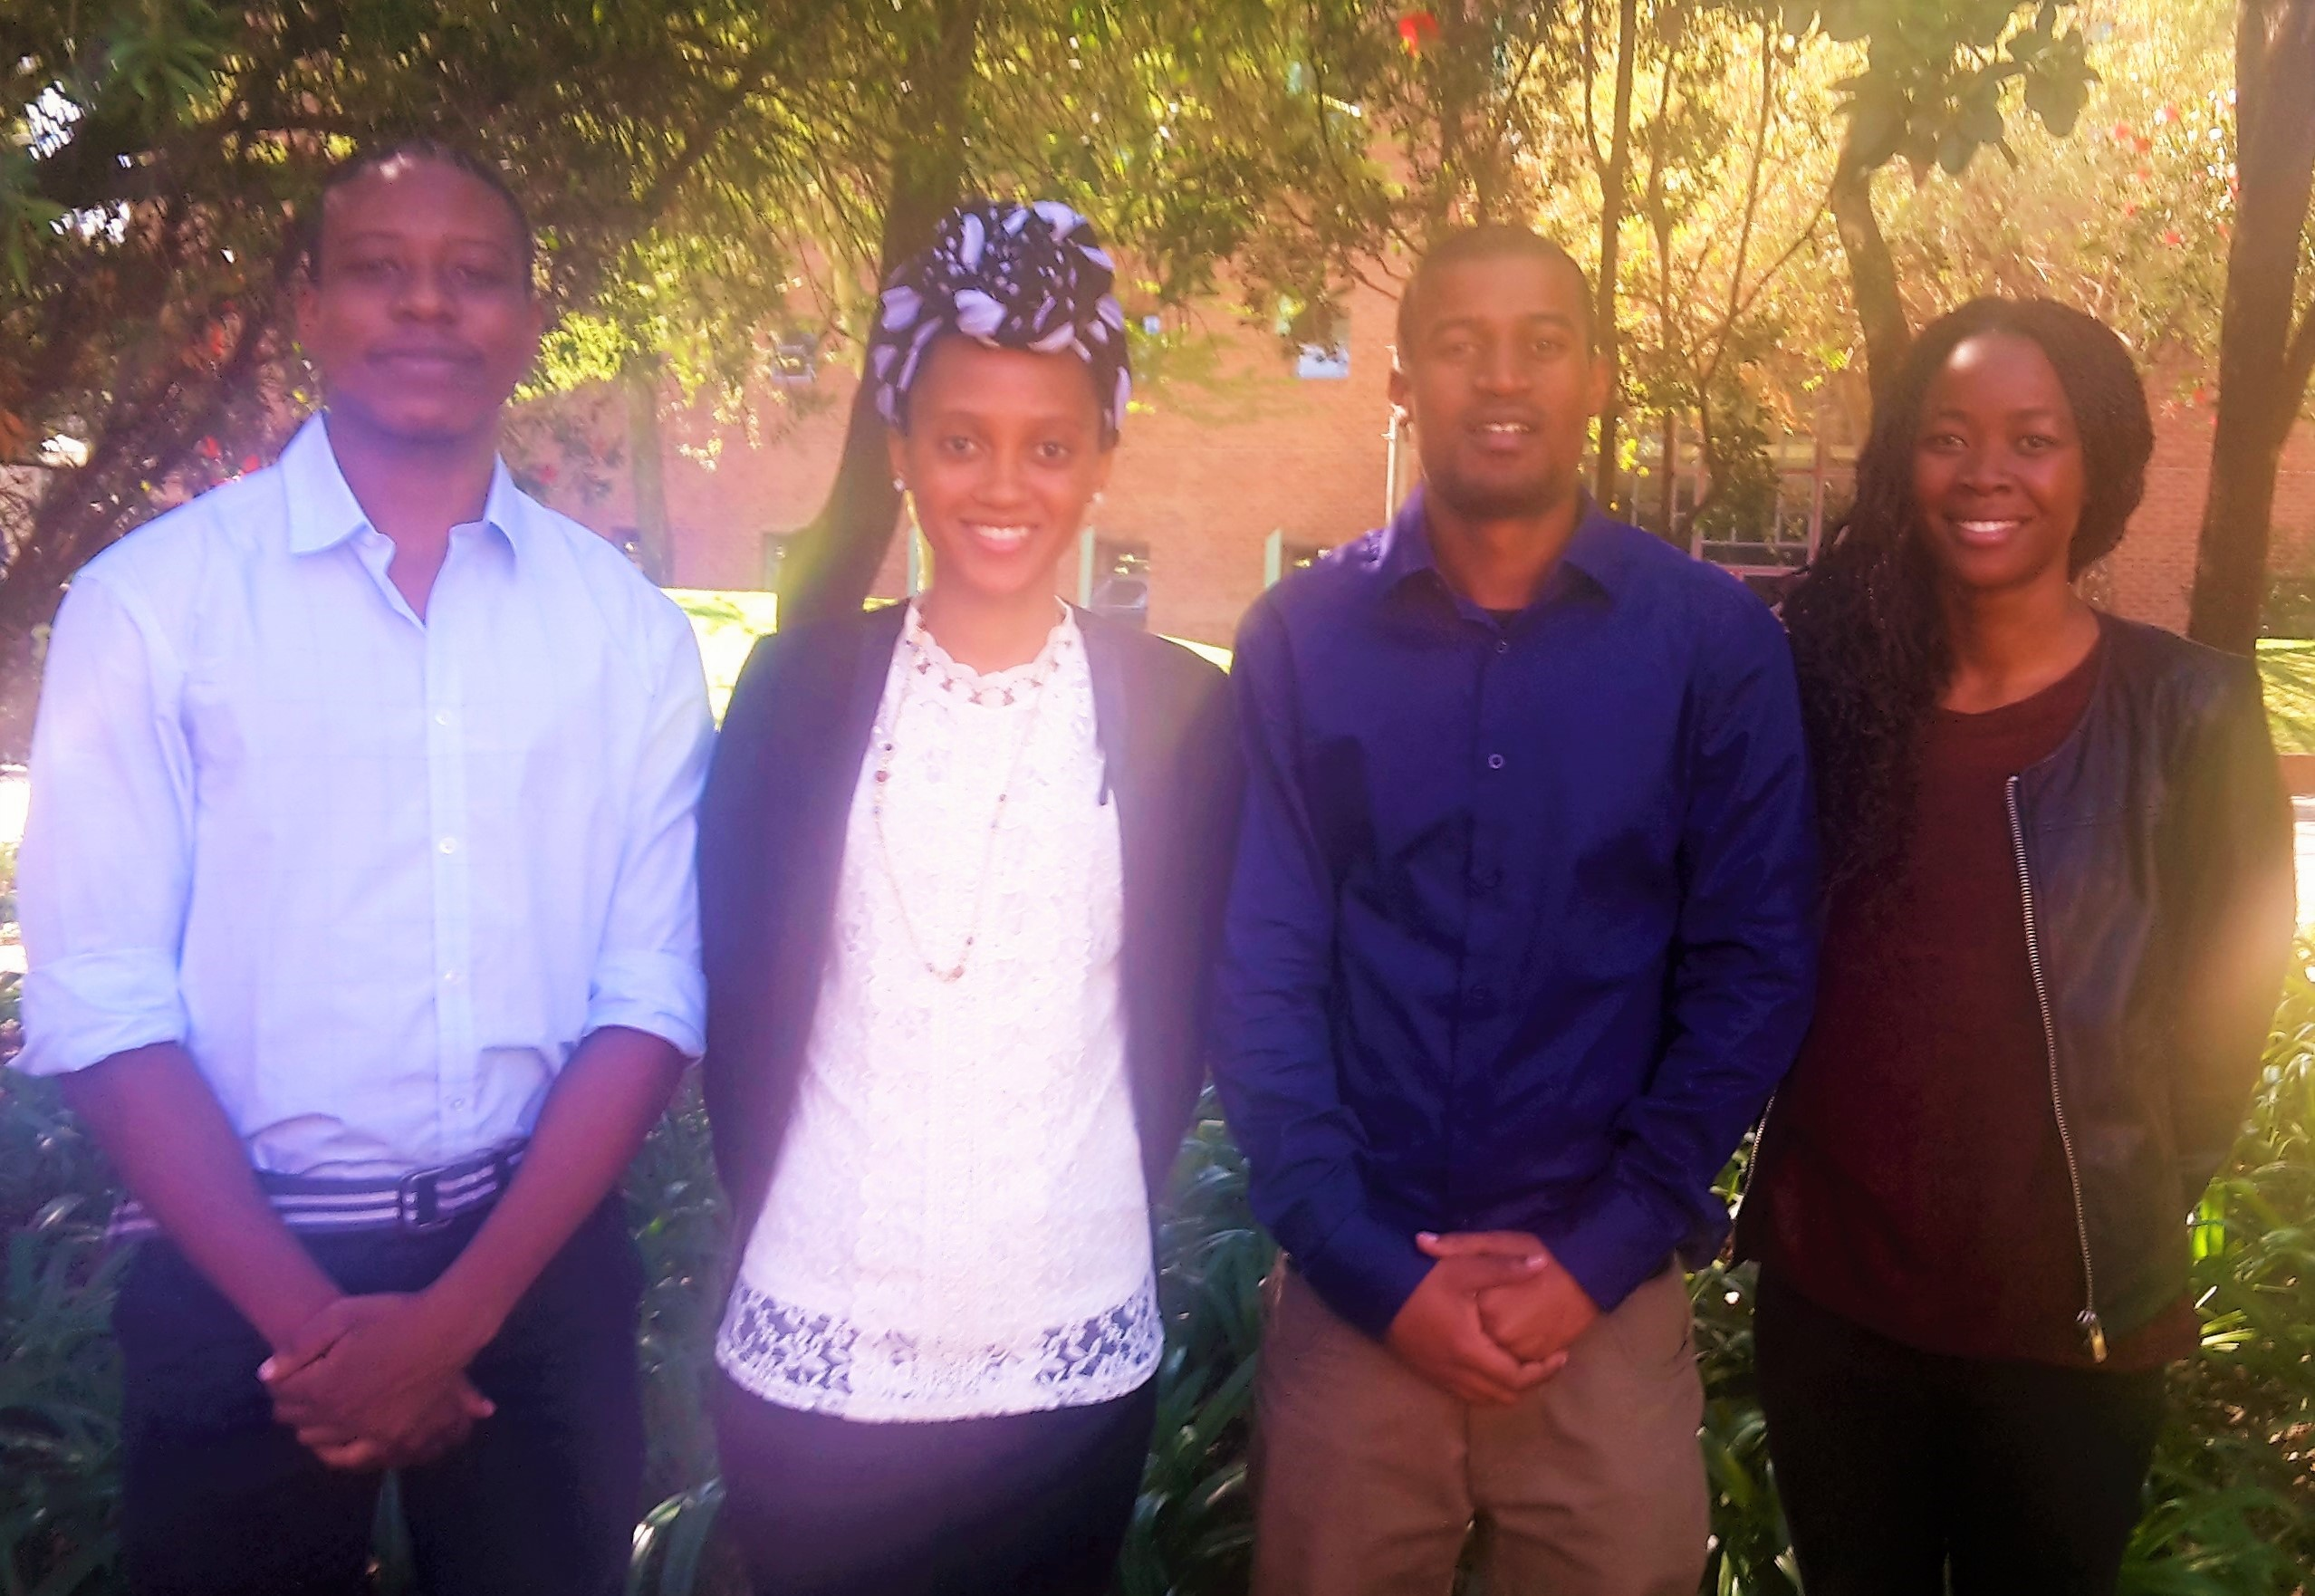
\includegraphics[width=3.5in]{./IMAPKD.jpg}

\vfill
% Bottom of the page
\end{center}
\end{titlepage}

\newpage
\section{Meet the Team Members}


%Priscilla Madigoe's Section - beginning

\begin{center}
{\Large Priscilla {Madigoe}} \\[0.3cm]
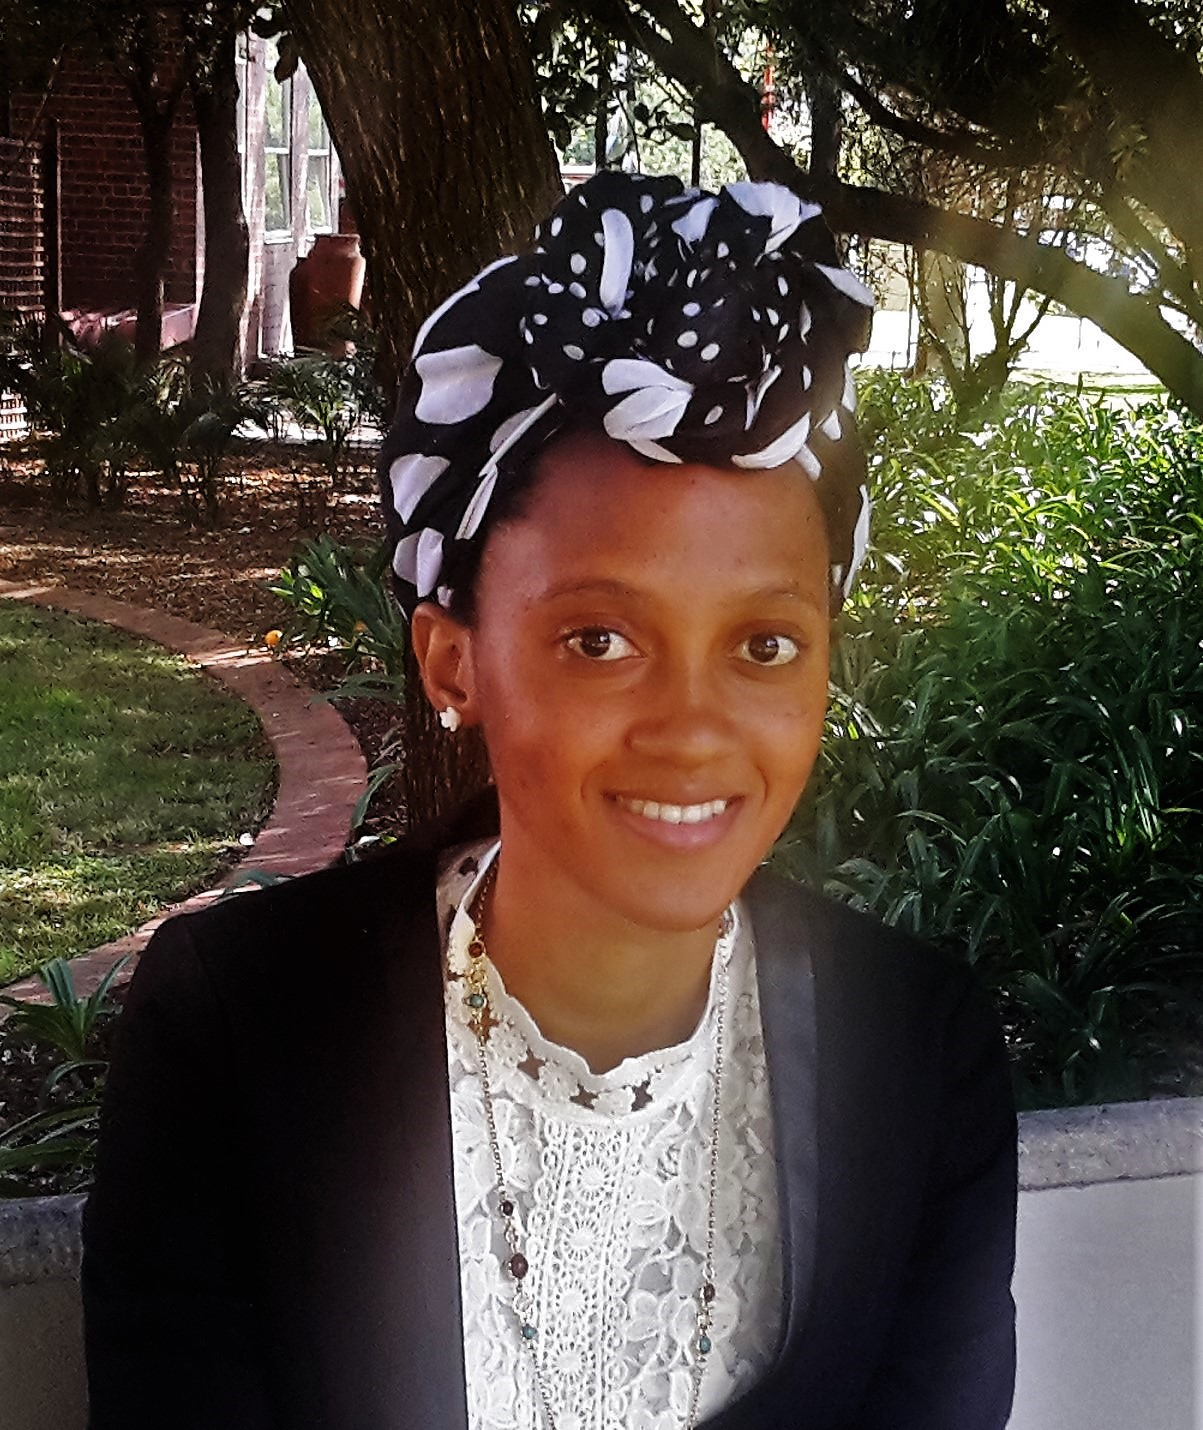
\includegraphics[width= 2in]{P.jpg}\\[0.4cm] 
\end{center}

\begin{itemize}
\item {\large \underline{\textbf{Interests}}}\\[0.2cm]
My interests include Computer Programming, Electronics, Computer Graphics, Robotics, travelling, photography, Anime, music, sports and reading novels.
\\
\item {\large \underline{\textbf{Technical Skills}}}

	\begin{itemize}
		\item Computer Programming with sound knowledge of Java, C/C++, MatLab, Assembler, WebGL and Web-related 			programming languages.
		\item Complex Problem-Solving using scientific and mathematical principles.
		\item System Analysis to determine how a computer software should behave in set conditions.
		\item Quality Control Analysis to evaluate the performance and quality of computer software.
	\end{itemize}
\bigskip
\item {\large \underline{\textbf{Past Experience}}}\\[0.2cm]
The Software Engineering module had a preparatory project called the Mini Project that was created to give students a real-world experience of software development. I took part in the project and I have learnt the process of software development, team work and different technologies used to develop computer software. 
\\
\item {\large \underline{\textbf{Non-Technical Skills}}}\\[0.2cm]
My non-technical skills include critical thinking, reading comprehension, writing, effective listening, social perceptiveness and active learning. 
\newpage
\item {\large \underline{\textbf{Reason for Interest in the Project}}}\\[0.2cm]
This project will give me an opportunity to use my knowledge gained in the Artificial Intelligence course to create intelligent algorithms for data collection, analysis and processing.

\end{itemize}
%Priscilla Madigoe's Section - end

\newpage

% Diana Obo's Section - start
\begin{center}
{\Large Diana {Obo}} \\[0.3cm]
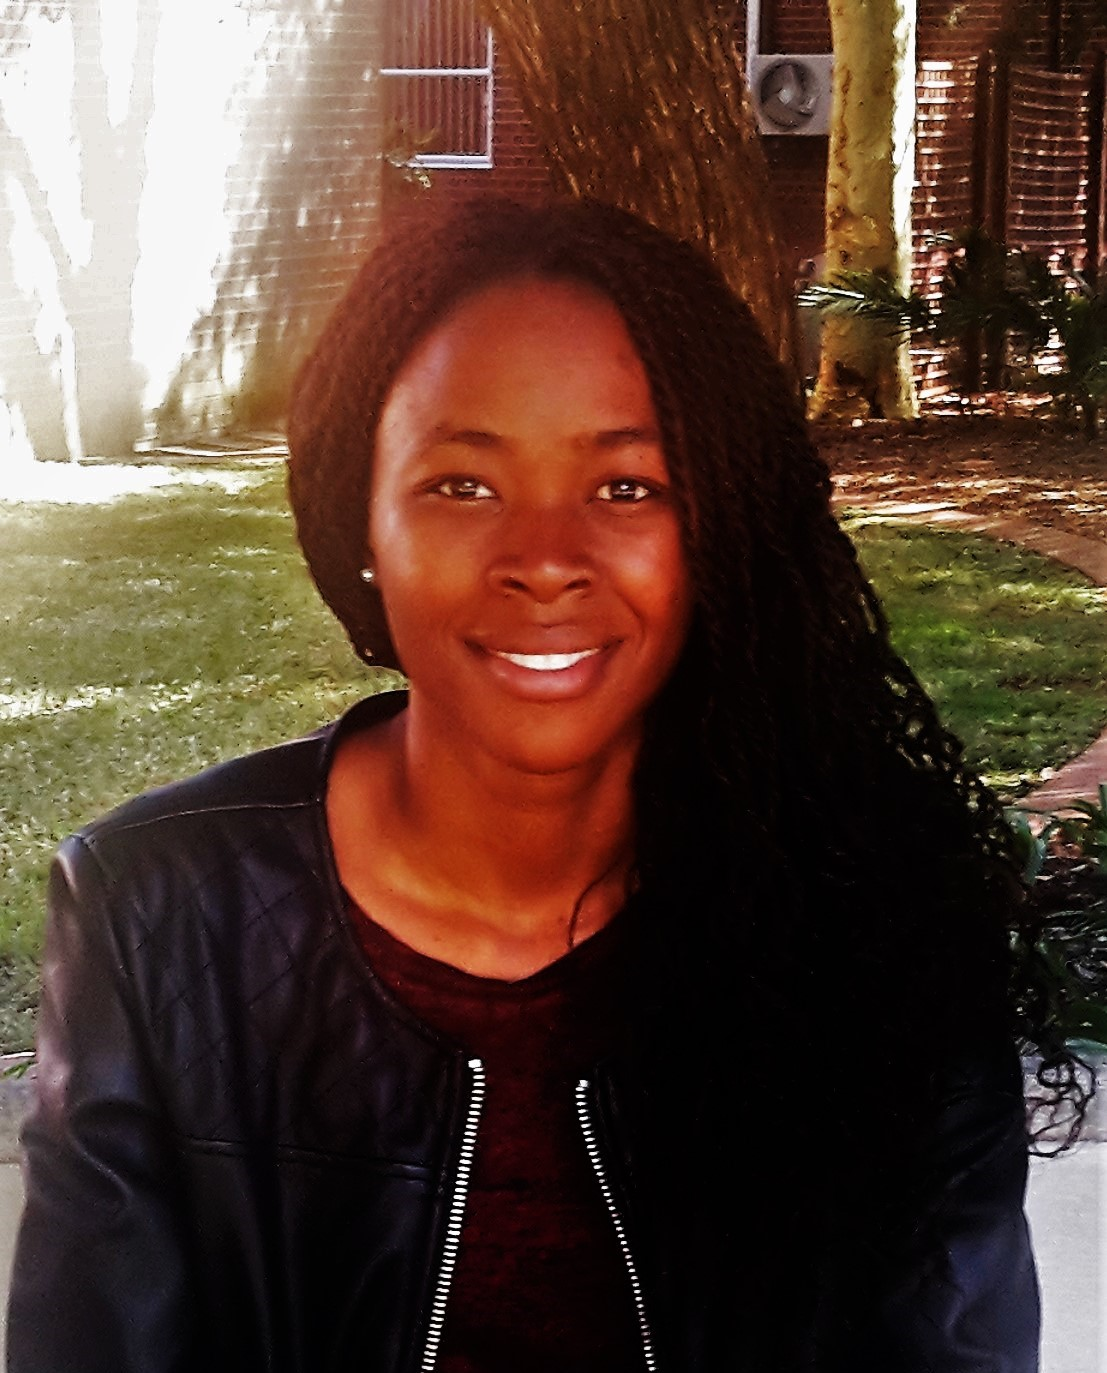
\includegraphics[width= 2in]{Diana.jpg}\\[0.4cm] 
\end{center}

\begin{itemize}
\item {\large \underline{\textbf{Interests}}}\\[0.2cm]
My interests are travelling, game development, Web development and Anime. I also enjoy learning about new technologies and watching a lot of discovery channels and documentaries.

\item {\large \underline{\textbf{Technical Skills}}}
	\begin{itemize}
		\item I have sound knowledge of Java, C++, HTML, CSS, Javascript, C\# and MatLab
		\item Mobile development (Android Studio) 
		\item 3DS MAX.
		\item Ember.js and  Handlebar.js
	\end{itemize}
\bigskip
\item {\large \underline{\textbf{Past Experience}}}
\begin{itemize}
\item I participated in this year's Standard Bank IT Challenge.
\item I did an internship at a small company named Lepsta where I did Web development.
\end{itemize}
\bigskip
\item {\large \underline{\textbf{Non-Technical Skills}}}
\begin{itemize}
\item Willingness to learn
\item Team player
\item Organised
\item Diligent
\item Reliable
\end{itemize}
\bigskip
\item {\Large \underline{\textbf{Reason for Interest in the Project}}}\\[0.2cm]
I feel this project will challenge me as a programmer and enable me to use all my knowledge that I have acquired as a computer programming student at The University of Pretoria and gain new programming skills.

\end{itemize}
%Diana Obo's Section - end

\newpage

% Kudzai Muranga's Section - start
\begin{center}
{\Large Kudzai {Muranga}} \\[0.3cm]
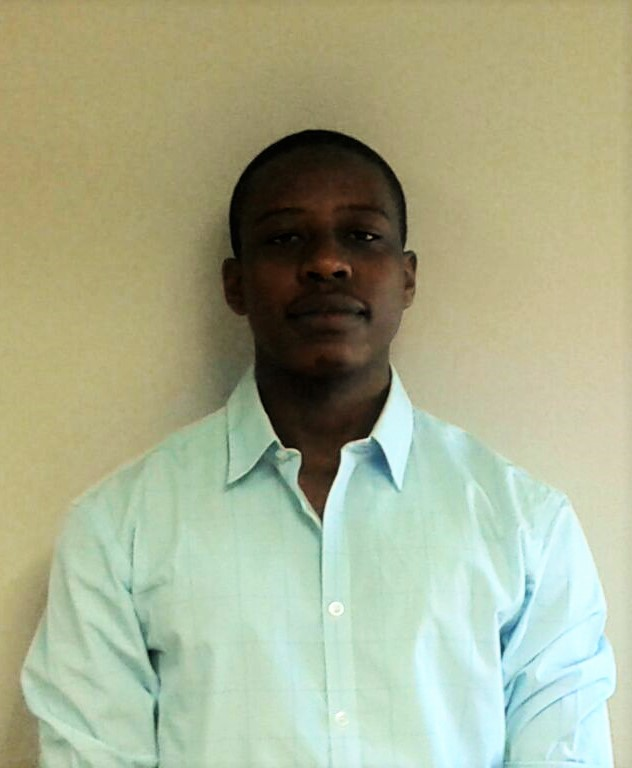
\includegraphics[width= 2in]{Kudzai.jpg}\\[0.4cm] 
\end{center}

\begin{itemize}
\item {\large \underline{\textbf{Interests}}}\\[0.2cm]
I am an avid reader. I love fantasy novels the most. I like to keep myself up to date with the current affairs of the world. I am also interested in learning anything new that concerns science, technology and business.
\\
\item {\large \underline{\textbf{Technical Skills}}}
	\begin{itemize}
		\item I have sound knowledge of Java, C++, HTML, CSS, Javascript, C\# and mobile development 
		\item Artificial Intelligence experience
		\item Business Management knowledge
		\item Project Management
	\end{itemize}
\bigskip
\item {\large \underline{\textbf{Past Experience}}}
\begin{itemize}
\item I have participated in the Standard Bank IT Challenge.
\item Invited to the Hello Group Open Day where I participated in a coding challenge using Java.
\end{itemize}
\bigskip
\item {\large \underline{\textbf{Non-Technical Skills}}}
\begin{itemize}
\item I am interested and open to learning new things
\item Disciplined
\item Organised
\item Critical Thinking
\end{itemize}
\bigskip
\item {\large \underline{\textbf{Reason for Interest in the Project}}}\\[0.2cm]
I am interested in this project because I feel that it would allow me to use my programming abilities extensively and teach me new and exciting skills.
% Kudzai Muranga's Section - end

\newpage
%Sandile Khumalo's Section - start
\end{itemize}
\begin{center}
{\Large Sandile {Khumalo}} \\[0.3cm]
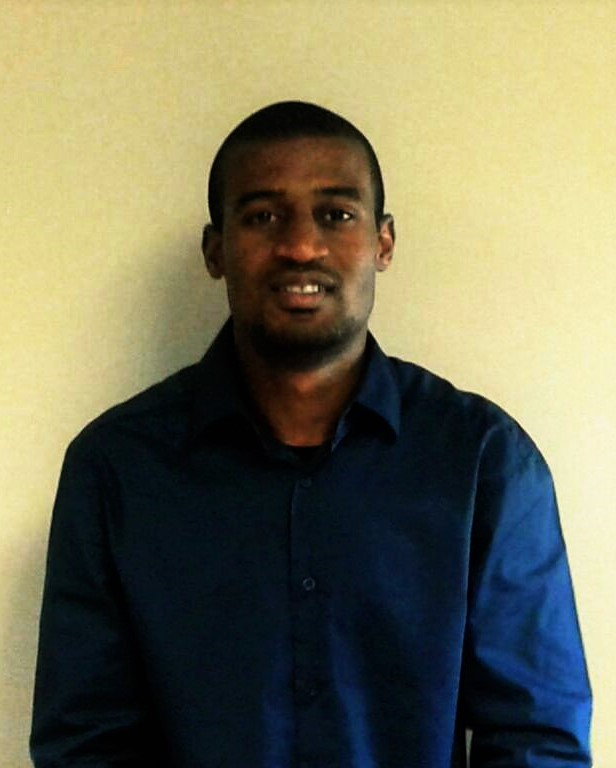
\includegraphics[width=2in]{Sandile.jpg}\\[0.4cm] 
\end{center}



\begin{itemize}
\item {\large \underline{\textbf{Interests}}}\\[0.2cm]
My interest are coding, reading on new and exciting technologies  and watching and reading about football. I also enjoy weightlifting.

\item {\large \underline{\textbf{Technical Skills}}}

	\begin{itemize}
		\item I am comfortable and have experience coding in these languages; C++, Java, C\#, PHP, HTML, JavaScript and Bash. I also have done 64 bit assembler language and I have experience in MINIX.
	\end{itemize}
\bigskip
\item {\large \underline{\textbf{Past Experience}}}\\[0.2cm]
I have done a project in my software development class that is similar. It incorporates  most of the technologies and frameworks used in the work place when developing big projects.
\\
\item {\large \underline{\textbf{Non-Technical Skills}}}\\[0.2cm]
 I am a hard working student. I am dedicated and I believe if there is a will, the is a way. This is especially true as a developer because most of the solutions are there and someone has done it before. It's a matter of good research and good understanding of the task at hand. I am willing to learn from every experience. 
\\
\item {\large \underline{\textbf{Reason for Interest in the Project}}}\\[0.2cm]
I like the technical part of this project. I'm looking forward to connecting different systems, especially where it incoparates everyday activities like swiping at the gates. I think this is a really good skill to have.

\end{itemize}

%Sandile Khumalo's Section - end
\newpage

%Project Execution
\section{Project Execution}

\begin{itemize}
\item {\large \underline{\textbf{Development Methodology}}}\\[0.2cm]
For this project, the following development methodology will be used:

	\begin{itemize}
 		\item \underline{Name:}
		\\[0.1cm]
		 Scrum
		\item  \underline{What is Scrum?}
		\\[0.1cm]
		Scrum is a lightweight management framework with broad applicability for managing \& controlling iterative \& 				incremental projects of all types (Takeuchi \& Nonaka, 1999).
		\item \underline{Why did we choose to use it?}
		\\[0.1cm]
		Because of all the potential additions that might occur at the different stages of development for this project, we 			have decided that Scrum is the best suited development methodology to use.
	\end{itemize}
\bigskip

\item {\large \underline{\textbf{Keeping Magna BC Informed}}}\\[0.2cm]
To keep the Magna BC informed about the project, we are going to use the following technologies and strategies:

	\begin{itemize}
	\item During the client meetings where we are going to discuss all aspects of the project.
	\item Send email to set up appointments.
	\item Use an application called Slack for general queries and updates.
	\end{itemize} 

\bigskip
\item {\large \underline{\textbf{Ideas to Solve Technical Problems for the Project}}}\\[0.2cm]
<<<<<<< HEAD

=======
\begin{enumerate}
    \item The data from all information sources should be sent to at the server in order to have it processed uniformly at a single point.
    \item The higher level performance areas can be specified as units of time. For example  they could measure a workers performance over a month, year or longer.
\end{enumerate}

\bigskip
>>>>>>> 27fbf9d02a0761a1430ebcc3f233246c3104d584
\item {\large \underline{\textbf{Possible Technologies to be Used}}}\\[0.2cm]
We are planning on using the following technologies for the project:
	\begin{itemize}
		\item \underline {Version Control:} Git
		\\
		\item  \underline{Unit Testing:} JUnit Framework
		\\
		\item We will use Maven for dependency management, plugin framework and support for modularization for 				projects.
		\\
		\item \underline{Front-end: Android} We will use the REST model to send data to and from the mobile application. 			The specific REST API framework we will use is GgaREST. It is free and easy to use.
	\end{itemize}

\bigskip
 \item {\large \underline{\textbf{What Magna BC will Receive}}}\\[0.2cm]
We will provide the project deliverables as expected. 
\end{itemize}
\end{document}

